\documentclass[12pt]{article}

\usepackage{sbc-template}

\usepackage{graphicx,url}

%\usepackage[brazil]{babel}   
\usepackage[latin1]{inputenc}  

     
\sloppy

\title{An�lise de desempenho do particionamento do algoritmo \textit{QuickSort} para os m�todos de \textit{Hoare} e \textit{Lomuto}}

\author{Eugenio Souza Carvalho\inst{1}, Hugo Santos Piauilino Neto\inst{1}}


\address{Departamento de Computa��o\\
	Universidade Federal do Piau�
  (UFPI)\\
  Teresina -- PI -- Brazil
  \email{\{hugos94,eugeniucarvalho\}@gmail.com}
}

\begin{document} 

\maketitle

\begin{abstract}
\end{abstract}
     
\begin{resumo} 
  Este trabalho apresenta uma an�lise de desempenho do particionamento do algoritmo de ordena��o \textit{QuickSort} para os m�todos propostos por \textit{Hoare} e \textit{Lomuto} \cite{cormen}, al�m de apresentar um resumo geral sobre a hist�ria e funcionamento do algoritmo de ordena��o. 
\end{resumo}


\section{Introdu��o}

\section{QuickSort}

\section{Resultados} \label{sec:firstpage}

\section{Conclus�o}



\begin{figure}[ht]
\centering
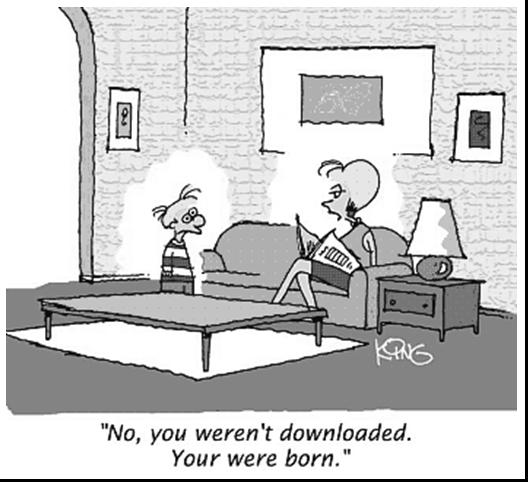
\includegraphics[width=.5\textwidth]{fig1.jpg}
\caption{A typical figure}
\label{fig:exampleFig1}
\end{figure}

\begin{figure}[ht]
\centering
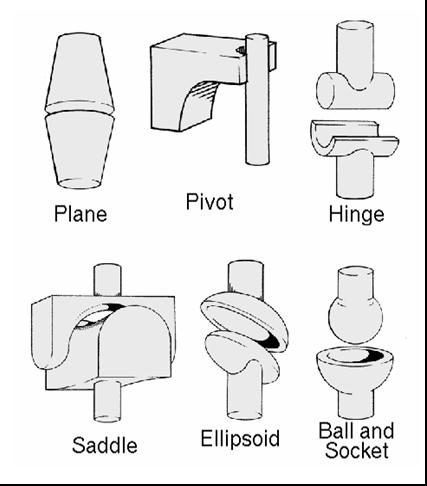
\includegraphics[width=.3\textwidth]{fig2.jpg}
\caption{This figure is an example of a figure caption taking more than one
  line and justified considering margins mentioned in Section~\ref{sec:figs}.}
\label{fig:exampleFig2}
\end{figure}


\bibliographystyle{sbc}
\bibliography{sbc-template}

\end{document}
